\documentclass{standalone}
\usepackage{tikz}
\usetikzlibrary{patterns, positioning}

\begin{document}
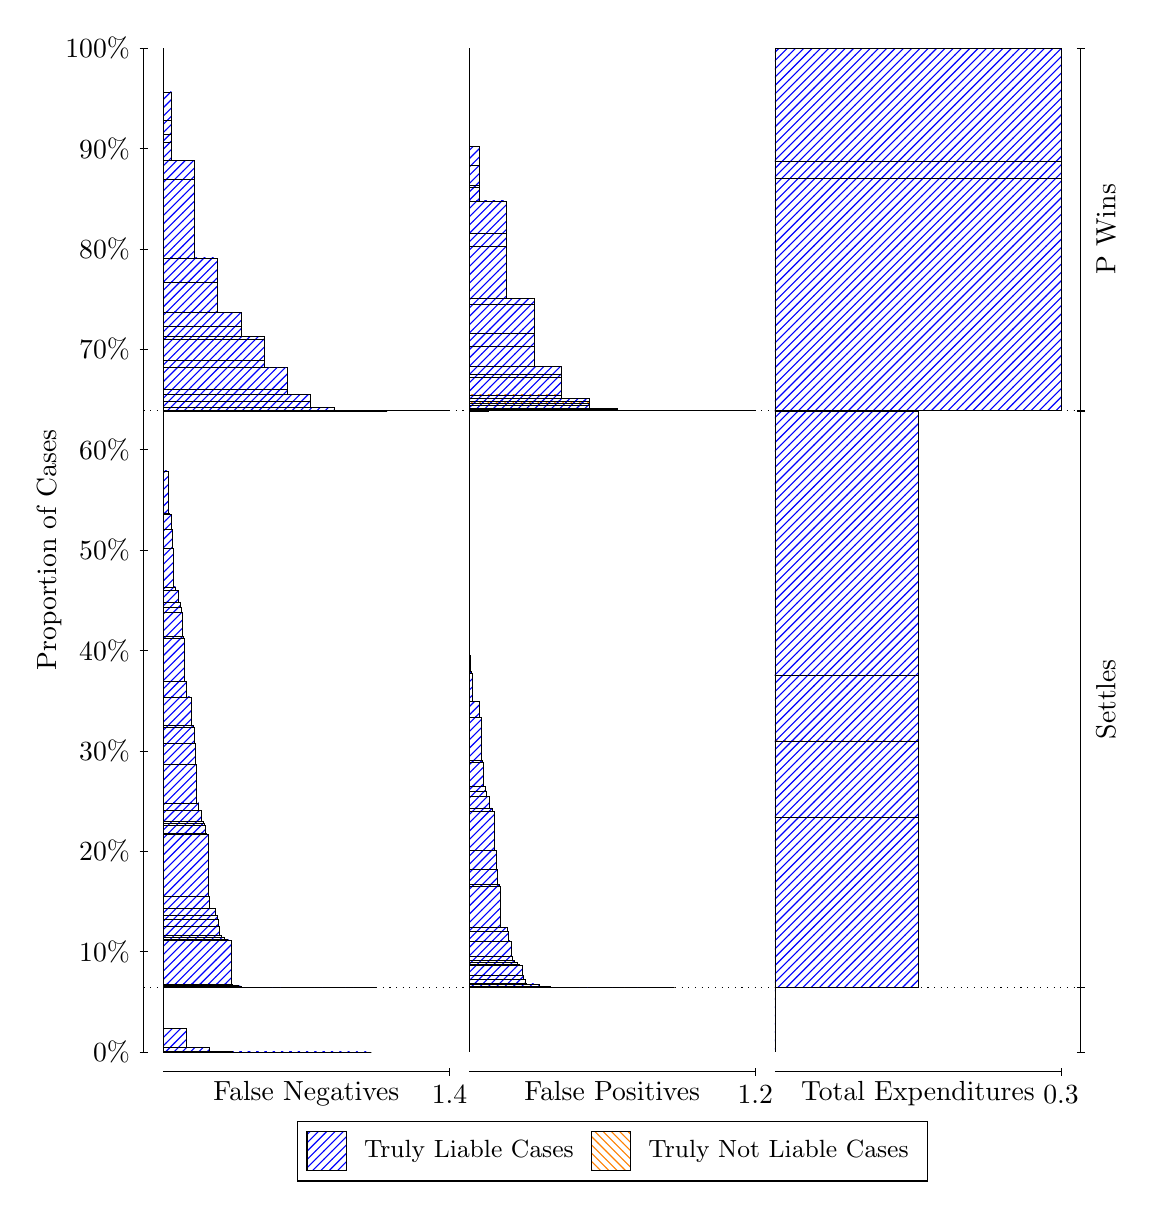
\begin{tikzpicture}
\draw[black, very thin] (1.5,1.75) -- (1.5,14.5);
\node[rotate=90, anchor=center] at (0.3, 8.125) {Proportion of Cases};
\draw[black, very thin] (1.45,1.75) -- (1.55,1.75);
\node[anchor=east] at (1.45, 1.75) {0\%};
\draw[black, very thin] (1.45,3.025) -- (1.55,3.025);
\node[anchor=east] at (1.45, 3.025) {10\%};
\draw[black, very thin] (1.45,4.3) -- (1.55,4.3);
\node[anchor=east] at (1.45, 4.3) {20\%};
\draw[black, very thin] (1.45,5.575) -- (1.55,5.575);
\node[anchor=east] at (1.45, 5.575) {30\%};
\draw[black, very thin] (1.45,6.85) -- (1.55,6.85);
\node[anchor=east] at (1.45, 6.85) {40\%};
\draw[black, very thin] (1.45,8.125) -- (1.55,8.125);
\node[anchor=east] at (1.45, 8.125) {50\%};
\draw[black, very thin] (1.45,9.4) -- (1.55,9.4);
\node[anchor=east] at (1.45, 9.4) {60\%};
\draw[black, very thin] (1.45,10.675) -- (1.55,10.675);
\node[anchor=east] at (1.45, 10.675) {70\%};
\draw[black, very thin] (1.45,11.95) -- (1.55,11.95);
\node[anchor=east] at (1.45, 11.95) {80\%};
\draw[black, very thin] (1.45,13.225) -- (1.55,13.225);
\node[anchor=east] at (1.45, 13.225) {90\%};
\draw[black, very thin] (1.45,14.5) -- (1.55,14.5);
\node[anchor=east] at (1.45, 14.5) {100\%};

\draw[black, very thin] (13.4,1.75) -- (13.4,14.5);
\draw[black, very thin] (13.35,1.75) -- (13.45,1.75);
\node[anchor=west] at (13.35, 1.75) {};
\draw[black, very thin] (13.35,2.5655) -- (13.45,2.5655);
\node[anchor=west] at (13.35, 2.5655) {};
\draw[black, very thin] (13.35,9.8923) -- (13.45,9.8923);
\node[anchor=west] at (13.35, 9.8923) {};
\draw[black, very thin] (13.35,9.8952) -- (13.45,9.8952);
\node[anchor=west] at (13.35, 9.8952) {};
\draw[black, very thin] (13.35,14.5) -- (13.45,14.5);
\node[anchor=west] at (13.35, 14.5) {};

\draw[black, very thin, pattern color=blue, pattern=north east lines] (1.75,1.75) rectangle (4.3924,1.75);
\draw[black, very thin, pattern color=blue, pattern=north east lines] (1.75,1.75) rectangle (4.0988,1.75);
\draw[black, very thin, pattern color=blue, pattern=north east lines] (1.75,1.75) rectangle (3.8052,1.75);
\draw[black, very thin, pattern color=blue, pattern=north east lines] (1.75,1.75) rectangle (3.5116,1.75);
\draw[black, very thin, pattern color=blue, pattern=north east lines] (1.75,1.75) rectangle (3.218,1.75);
\draw[black, very thin, pattern color=blue, pattern=north east lines] (1.75,1.75) rectangle (2.9244,1.7502);
\draw[black, very thin, pattern color=blue, pattern=north east lines] (1.75,1.7502) rectangle (2.6308,1.7558);
\draw[black, very thin, pattern color=blue, pattern=north east lines] (1.75,1.7558) rectangle (2.3372,1.8123);
\draw[black, very thin, pattern color=blue, pattern=north east lines] (1.75,1.8123) rectangle (2.0436,2.0523);
\draw[black, very thin, pattern color=orange, pattern=north west lines] (1.75,2.0523) rectangle (1.75,2.0523);
\draw[black, very thin, pattern color=blue, pattern=north east lines] (1.75,2.0523) rectangle (1.75,2.5655);
\draw[black, very thin, pattern color=blue, pattern=north east lines] (1.75,2.5655) rectangle (4.4585,2.5655);
\draw[black, very thin, pattern color=blue, pattern=north east lines] (1.75,2.5655) rectangle (4.3264,2.5655);
\draw[black, very thin, pattern color=blue, pattern=north east lines] (1.75,2.5655) rectangle (4.1942,2.5655);
\draw[black, very thin, pattern color=blue, pattern=north east lines] (1.75,2.5655) rectangle (4.1649,2.5655);
\draw[black, very thin, pattern color=blue, pattern=north east lines] (1.75,2.5655) rectangle (4.0621,2.5655);
\draw[black, very thin, pattern color=blue, pattern=north east lines] (1.75,2.5655) rectangle (4.0328,2.5655);
\draw[black, very thin, pattern color=blue, pattern=north east lines] (1.75,2.5655) rectangle (3.93,2.5655);
\draw[black, very thin, pattern color=blue, pattern=north east lines] (1.75,2.5655) rectangle (3.9006,2.5655);
\draw[black, very thin, pattern color=blue, pattern=north east lines] (1.75,2.5655) rectangle (3.8713,2.5655);
\draw[black, very thin, pattern color=blue, pattern=north east lines] (1.75,2.5655) rectangle (3.7979,2.5655);
\draw[black, very thin, pattern color=blue, pattern=north east lines] (1.75,2.5655) rectangle (3.7685,2.5655);
\draw[black, very thin, pattern color=blue, pattern=north east lines] (1.75,2.5655) rectangle (3.7392,2.5655);
\draw[black, very thin, pattern color=blue, pattern=north east lines] (1.75,2.5655) rectangle (3.6658,2.5655);
\draw[black, very thin, pattern color=blue, pattern=north east lines] (1.75,2.5655) rectangle (3.6658,2.5655);
\draw[black, very thin, pattern color=blue, pattern=north east lines] (1.75,2.5655) rectangle (3.6364,2.5655);
\draw[black, very thin, pattern color=blue, pattern=north east lines] (1.75,2.5655) rectangle (3.607,2.5655);
\draw[black, very thin, pattern color=blue, pattern=north east lines] (1.75,2.5655) rectangle (3.5777,2.5655);
\draw[black, very thin, pattern color=blue, pattern=north east lines] (1.75,2.5655) rectangle (3.5336,2.5655);
\draw[black, very thin, pattern color=blue, pattern=north east lines] (1.75,2.5655) rectangle (3.5043,2.5655);
\draw[black, very thin, pattern color=blue, pattern=north east lines] (1.75,2.5655) rectangle (3.4749,2.5655);
\draw[black, very thin, pattern color=blue, pattern=north east lines] (1.75,2.5655) rectangle (3.4456,2.5655);
\draw[black, very thin, pattern color=blue, pattern=north east lines] (1.75,2.5655) rectangle (3.4015,2.5655);
\draw[black, very thin, pattern color=blue, pattern=north east lines] (1.75,2.5655) rectangle (3.3722,2.5655);
\draw[black, very thin, pattern color=blue, pattern=north east lines] (1.75,2.5655) rectangle (3.3722,2.5655);
\draw[black, very thin, pattern color=blue, pattern=north east lines] (1.75,2.5655) rectangle (3.3428,2.5655);
\draw[black, very thin, pattern color=blue, pattern=north east lines] (1.75,2.5655) rectangle (3.3134,2.5655);
\draw[black, very thin, pattern color=blue, pattern=north east lines] (1.75,2.5655) rectangle (3.2841,2.5655);
\draw[black, very thin, pattern color=blue, pattern=north east lines] (1.75,2.5655) rectangle (3.2694,2.5655);
\draw[black, very thin, pattern color=blue, pattern=north east lines] (1.75,2.5655) rectangle (3.24,2.5655);
\draw[black, very thin, pattern color=blue, pattern=north east lines] (1.75,2.5655) rectangle (3.2107,2.5655);
\draw[black, very thin, pattern color=blue, pattern=north east lines] (1.75,2.5655) rectangle (3.1813,2.5655);
\draw[black, very thin, pattern color=blue, pattern=north east lines] (1.75,2.5655) rectangle (3.152,2.5655);
\draw[black, very thin, pattern color=blue, pattern=north east lines] (1.75,2.5655) rectangle (3.1373,2.5655);
\draw[black, very thin, pattern color=blue, pattern=north east lines] (1.75,2.5655) rectangle (3.1079,2.5655);
\draw[black, very thin, pattern color=blue, pattern=north east lines] (1.75,2.5655) rectangle (3.0786,2.5655);
\draw[black, very thin, pattern color=blue, pattern=north east lines] (1.75,2.5655) rectangle (3.0492,2.5655);
\draw[black, very thin, pattern color=blue, pattern=north east lines] (1.75,2.5655) rectangle (3.0198,2.5656);
\draw[black, very thin, pattern color=blue, pattern=north east lines] (1.75,2.5656) rectangle (3.0052,2.5656);
\draw[black, very thin, pattern color=blue, pattern=north east lines] (1.75,2.5656) rectangle (2.9905,2.5656);
\draw[black, very thin, pattern color=blue, pattern=north east lines] (1.75,2.5656) rectangle (2.9758,2.5656);
\draw[black, very thin, pattern color=blue, pattern=north east lines] (1.75,2.5656) rectangle (2.9464,2.5656);
\draw[black, very thin, pattern color=blue, pattern=north east lines] (1.75,2.5656) rectangle (2.9171,2.5661);
\draw[black, very thin, pattern color=blue, pattern=north east lines] (1.75,2.5661) rectangle (2.8877,2.5662);
\draw[black, very thin, pattern color=blue, pattern=north east lines] (1.75,2.5662) rectangle (2.873,2.5663);
\draw[black, very thin, pattern color=blue, pattern=north east lines] (1.75,2.5663) rectangle (2.8584,2.5663);
\draw[black, very thin, pattern color=blue, pattern=north east lines] (1.75,2.5663) rectangle (2.8437,2.5663);
\draw[black, very thin, pattern color=blue, pattern=north east lines] (1.75,2.5663) rectangle (2.8143,2.5669);
\draw[black, very thin, pattern color=blue, pattern=north east lines] (1.75,2.5669) rectangle (2.7849,2.5688);
\draw[black, very thin, pattern color=blue, pattern=north east lines] (1.75,2.5688) rectangle (2.7849,2.5688);
\draw[black, very thin, pattern color=blue, pattern=north east lines] (1.75,2.5688) rectangle (2.7556,2.5745);
\draw[black, very thin, pattern color=blue, pattern=north east lines] (1.75,2.5745) rectangle (2.7409,2.5858);
\draw[black, very thin, pattern color=blue, pattern=north east lines] (1.75,2.5858) rectangle (2.7262,2.5881);
\draw[black, very thin, pattern color=blue, pattern=north east lines] (1.75,2.5881) rectangle (2.7115,2.5884);
\draw[black, very thin, pattern color=blue, pattern=north east lines] (1.75,2.5884) rectangle (2.6969,2.5927);
\draw[black, very thin, pattern color=blue, pattern=north east lines] (1.75,2.5927) rectangle (2.6822,2.5929);
\draw[black, very thin, pattern color=blue, pattern=north east lines] (1.75,2.5929) rectangle (2.6528,2.5929);
\draw[black, very thin, pattern color=blue, pattern=north east lines] (1.75,2.5929) rectangle (2.6235,2.6134);
\draw[black, very thin, pattern color=blue, pattern=north east lines] (1.75,2.6134) rectangle (2.6088,3.1659);
\draw[black, very thin, pattern color=blue, pattern=north east lines] (1.75,3.1659) rectangle (2.5941,3.1689);
\draw[black, very thin, pattern color=blue, pattern=north east lines] (1.75,3.1689) rectangle (2.5794,3.1748);
\draw[black, very thin, pattern color=blue, pattern=north east lines] (1.75,3.1748) rectangle (2.5647,3.1769);
\draw[black, very thin, pattern color=blue, pattern=north east lines] (1.75,3.1769) rectangle (2.5501,3.1788);
\draw[black, very thin, pattern color=blue, pattern=north east lines] (1.75,3.1788) rectangle (2.5207,3.2005);
\draw[black, very thin, pattern color=blue, pattern=north east lines] (1.75,3.2005) rectangle (2.4913,3.233);
\draw[black, very thin, pattern color=blue, pattern=north east lines] (1.75,3.233) rectangle (2.4913,3.2331);
\draw[black, very thin, pattern color=blue, pattern=north east lines] (1.75,3.2331) rectangle (2.462,3.35);
\draw[black, very thin, pattern color=blue, pattern=north east lines] (1.75,3.35) rectangle (2.4473,3.4345);
\draw[black, very thin, pattern color=blue, pattern=north east lines] (1.75,3.4345) rectangle (2.4326,3.4827);
\draw[black, very thin, pattern color=blue, pattern=north east lines] (1.75,3.4827) rectangle (2.4179,3.488);
\draw[black, very thin, pattern color=blue, pattern=north east lines] (1.75,3.488) rectangle (2.4033,3.5719);
\draw[black, very thin, pattern color=blue, pattern=north east lines] (1.75,3.5719) rectangle (2.3886,3.5744);
\draw[black, very thin, pattern color=blue, pattern=north east lines] (1.75,3.5744) rectangle (2.3592,3.5744);
\draw[black, very thin, pattern color=blue, pattern=north east lines] (1.75,3.5744) rectangle (2.3299,3.722);
\draw[black, very thin, pattern color=blue, pattern=north east lines] (1.75,3.722) rectangle (2.3152,4.5144);
\draw[black, very thin, pattern color=blue, pattern=north east lines] (1.75,4.5144) rectangle (2.3005,4.5335);
\draw[black, very thin, pattern color=blue, pattern=north east lines] (1.75,4.5335) rectangle (2.2858,4.6279);
\draw[black, very thin, pattern color=blue, pattern=north east lines] (1.75,4.6279) rectangle (2.2711,4.6524);
\draw[black, very thin, pattern color=blue, pattern=north east lines] (1.75,4.6524) rectangle (2.2565,4.682);
\draw[black, very thin, pattern color=blue, pattern=north east lines] (1.75,4.682) rectangle (2.2271,4.8206);
\draw[black, very thin, pattern color=blue, pattern=north east lines] (1.75,4.8206) rectangle (2.1977,4.9137);
\draw[black, very thin, pattern color=blue, pattern=north east lines] (1.75,4.9137) rectangle (2.1977,4.9142);
\draw[black, very thin, pattern color=blue, pattern=north east lines] (1.75,4.9142) rectangle (2.1684,5.4048);
\draw[black, very thin, pattern color=blue, pattern=north east lines] (1.75,5.4048) rectangle (2.1537,5.6723);
\draw[black, very thin, pattern color=blue, pattern=north east lines] (1.75,5.6723) rectangle (2.139,5.872);
\draw[black, very thin, pattern color=blue, pattern=north east lines] (1.75,5.872) rectangle (2.1243,5.8958);
\draw[black, very thin, pattern color=blue, pattern=north east lines] (1.75,5.8958) rectangle (2.1097,6.2535);
\draw[black, very thin, pattern color=blue, pattern=north east lines] (1.75,6.2535) rectangle (2.095,6.2592);
\draw[black, very thin, pattern color=blue, pattern=north east lines] (1.75,6.2592) rectangle (2.0656,6.2592);
\draw[black, very thin, pattern color=blue, pattern=north east lines] (1.75,6.2592) rectangle (2.0363,6.4519);
\draw[black, very thin, pattern color=blue, pattern=north east lines] (1.75,6.4519) rectangle (2.0216,7.0045);
\draw[black, very thin, pattern color=blue, pattern=north east lines] (1.75,7.0045) rectangle (2.0069,7.0247);
\draw[black, very thin, pattern color=blue, pattern=north east lines] (1.75,7.0247) rectangle (1.9922,7.3298);
\draw[black, very thin, pattern color=blue, pattern=north east lines] (1.75,7.3298) rectangle (1.9775,7.3914);
\draw[black, very thin, pattern color=blue, pattern=north east lines] (1.75,7.3914) rectangle (1.9629,7.4659);
\draw[black, very thin, pattern color=blue, pattern=north east lines] (1.75,7.4659) rectangle (1.9335,7.6073);
\draw[black, very thin, pattern color=blue, pattern=north east lines] (1.75,7.6073) rectangle (1.9041,7.6556);
\draw[black, very thin, pattern color=blue, pattern=north east lines] (1.75,7.6556) rectangle (1.9041,7.6561);
\draw[black, very thin, pattern color=blue, pattern=north east lines] (1.75,7.6561) rectangle (1.8748,8.1431);
\draw[black, very thin, pattern color=blue, pattern=north east lines] (1.75,8.1431) rectangle (1.8601,8.3888);
\draw[black, very thin, pattern color=blue, pattern=north east lines] (1.75,8.3888) rectangle (1.8454,8.577);
\draw[black, very thin, pattern color=blue, pattern=north east lines] (1.75,8.577) rectangle (1.8307,8.5976);
\draw[black, very thin, pattern color=blue, pattern=north east lines] (1.75,8.5976) rectangle (1.8161,9.1273);
\draw[black, very thin, pattern color=blue, pattern=north east lines] (1.75,9.1273) rectangle (1.8014,9.1297);
\draw[black, very thin, pattern color=blue, pattern=north east lines] (1.75,9.1297) rectangle (1.772,9.1297);
\draw[black, very thin, pattern color=orange, pattern=north west lines] (1.75,9.1297) rectangle (1.75,9.1297);
\draw[black, very thin, pattern color=blue, pattern=north east lines] (1.75,9.1297) rectangle (1.75,9.8923);
\draw[black, very thin, pattern color=blue, pattern=north east lines] (1.75,9.8923) rectangle (4.5906,9.8923);
\draw[black, very thin, pattern color=blue, pattern=north east lines] (1.75,9.8923) rectangle (4.297,9.8923);
\draw[black, very thin, pattern color=blue, pattern=north east lines] (1.75,9.8923) rectangle (4.0034,9.8923);
\draw[black, very thin, pattern color=blue, pattern=north east lines] (1.75,9.8923) rectangle (3.7098,9.8923);
\draw[black, very thin, pattern color=blue, pattern=north east lines] (1.75,9.8923) rectangle (3.4162,9.8923);
\draw[black, very thin, pattern color=blue, pattern=north east lines] (1.75,9.8923) rectangle (3.1226,9.8923);
\draw[black, very thin, pattern color=blue, pattern=north east lines] (1.75,9.8923) rectangle (2.829,9.8923);
\draw[black, very thin, pattern color=blue, pattern=north east lines] (1.75,9.8923) rectangle (2.5354,9.8927);
\draw[black, very thin, pattern color=blue, pattern=north east lines] (1.75,9.8927) rectangle (2.2418,9.8939);
\draw[black, very thin, pattern color=blue, pattern=north east lines] (1.75,9.8939) rectangle (1.9482,9.8952);
\draw[black, very thin, pattern color=orange, pattern=north west lines] (1.75,9.8952) rectangle (1.75,9.8952);
\draw[black, very thin, pattern color=blue, pattern=north east lines] (1.75,9.8952) rectangle (5.3833,9.8952);
\draw[black, very thin, pattern color=blue, pattern=north east lines] (1.75,9.8952) rectangle (5.0897,9.8952);
\draw[black, very thin, pattern color=blue, pattern=north east lines] (1.75,9.8952) rectangle (4.7961,9.8952);
\draw[black, very thin, pattern color=blue, pattern=north east lines] (1.75,9.8952) rectangle (4.5025,9.8954);
\draw[black, very thin, pattern color=blue, pattern=north east lines] (1.75,9.8954) rectangle (4.5025,9.8955);
\draw[black, very thin, pattern color=blue, pattern=north east lines] (1.75,9.8955) rectangle (4.4952,9.8955);
\draw[black, very thin, pattern color=blue, pattern=north east lines] (1.75,9.8955) rectangle (4.2089,9.8994);
\draw[black, very thin, pattern color=blue, pattern=north east lines] (1.75,9.8994) rectangle (4.2016,9.8994);
\draw[black, very thin, pattern color=blue, pattern=north east lines] (1.75,9.8994) rectangle (4.2016,9.8994);
\draw[black, very thin, pattern color=blue, pattern=north east lines] (1.75,9.8994) rectangle (3.9153,9.9327);
\draw[black, very thin, pattern color=blue, pattern=north east lines] (1.75,9.9327) rectangle (3.908,9.9327);
\draw[black, very thin, pattern color=blue, pattern=north east lines] (1.75,9.9327) rectangle (3.6217,10.016);
\draw[black, very thin, pattern color=blue, pattern=north east lines] (1.75,10.016) rectangle (3.6217,10.097);
\draw[black, very thin, pattern color=blue, pattern=north east lines] (1.75,10.097) rectangle (3.6144,10.097);
\draw[black, very thin, pattern color=blue, pattern=north east lines] (1.75,10.097) rectangle (3.6144,10.097);
\draw[black, very thin, pattern color=blue, pattern=north east lines] (1.75,10.097) rectangle (3.3281,10.169);
\draw[black, very thin, pattern color=blue, pattern=north east lines] (1.75,10.169) rectangle (3.3281,10.449);
\draw[black, very thin, pattern color=blue, pattern=north east lines] (1.75,10.449) rectangle (3.3208,10.449);
\draw[black, very thin, pattern color=blue, pattern=north east lines] (1.75,10.449) rectangle (3.0345,10.537);
\draw[black, very thin, pattern color=blue, pattern=north east lines] (1.75,10.537) rectangle (3.0345,10.801);
\draw[black, very thin, pattern color=blue, pattern=north east lines] (1.75,10.801) rectangle (3.0345,10.833);
\draw[black, very thin, pattern color=blue, pattern=north east lines] (1.75,10.833) rectangle (3.0272,10.834);
\draw[black, very thin, pattern color=blue, pattern=north east lines] (1.75,10.834) rectangle (3.0272,10.835);
\draw[black, very thin, pattern color=blue, pattern=north east lines] (1.75,10.835) rectangle (2.7409,10.969);
\draw[black, very thin, pattern color=blue, pattern=north east lines] (1.75,10.969) rectangle (2.7336,11.142);
\draw[black, very thin, pattern color=blue, pattern=north east lines] (1.75,11.142) rectangle (2.4473,11.142);
\draw[black, very thin, pattern color=blue, pattern=north east lines] (1.75,11.142) rectangle (2.4473,11.148);
\draw[black, very thin, pattern color=blue, pattern=north east lines] (1.75,11.148) rectangle (2.4473,11.148);
\draw[black, very thin, pattern color=blue, pattern=north east lines] (1.75,11.148) rectangle (2.44,11.529);
\draw[black, very thin, pattern color=blue, pattern=north east lines] (1.75,11.529) rectangle (2.44,11.836);
\draw[black, very thin, pattern color=blue, pattern=north east lines] (1.75,11.836) rectangle (2.1537,11.836);
\draw[black, very thin, pattern color=blue, pattern=north east lines] (1.75,11.836) rectangle (2.1537,11.836);
\draw[black, very thin, pattern color=blue, pattern=north east lines] (1.75,11.836) rectangle (2.1464,12.831);
\draw[black, very thin, pattern color=blue, pattern=north east lines] (1.75,12.831) rectangle (2.1464,13.076);
\draw[black, very thin, pattern color=blue, pattern=north east lines] (1.75,13.076) rectangle (1.8601,13.076);
\draw[black, very thin, pattern color=blue, pattern=north east lines] (1.75,13.076) rectangle (1.8601,13.076);
\draw[black, very thin, pattern color=blue, pattern=north east lines] (1.75,13.076) rectangle (1.8528,13.308);
\draw[black, very thin, pattern color=blue, pattern=north east lines] (1.75,13.308) rectangle (1.8528,13.4);
\draw[black, very thin, pattern color=blue, pattern=north east lines] (1.75,13.4) rectangle (1.8528,13.582);
\draw[black, very thin, pattern color=blue, pattern=north east lines] (1.75,13.582) rectangle (1.8528,13.942);
\draw[black, very thin, pattern color=orange, pattern=north west lines] (1.75,13.942) rectangle (1.75,13.942);
\draw[black, very thin, pattern color=blue, pattern=north east lines] (1.75,13.942) rectangle (1.75,14.5);
\draw[black, very thin, pattern color=orange, pattern=north west lines] (5.6333,1.75) rectangle (5.6333,1.75);
\draw[black, very thin, pattern color=blue, pattern=north east lines] (5.6333,1.75) rectangle (5.6333,2.5655);
\draw[black, very thin, pattern color=orange, pattern=north west lines] (5.6333,2.5655) rectangle (8.2399,2.5655);
\draw[black, very thin, pattern color=blue, pattern=north east lines] (5.6333,2.5655) rectangle (8.2399,2.5655);
\draw[black, very thin, pattern color=orange, pattern=north west lines] (5.6333,2.5655) rectangle (8.0819,2.5655);
\draw[black, very thin, pattern color=blue, pattern=north east lines] (5.6333,2.5655) rectangle (8.0819,2.5655);
\draw[black, very thin, pattern color=orange, pattern=north west lines] (5.6333,2.5655) rectangle (7.9239,2.5655);
\draw[black, very thin, pattern color=blue, pattern=north east lines] (5.6333,2.5655) rectangle (7.9239,2.5655);
\draw[black, very thin, pattern color=blue, pattern=north east lines] (5.6333,2.5655) rectangle (7.8888,2.5655);
\draw[black, very thin, pattern color=orange, pattern=north west lines] (5.6333,2.5655) rectangle (7.7659,2.5655);
\draw[black, very thin, pattern color=blue, pattern=north east lines] (5.6333,2.5655) rectangle (7.7659,2.5655);
\draw[black, very thin, pattern color=blue, pattern=north east lines] (5.6333,2.5655) rectangle (7.7308,2.5655);
\draw[black, very thin, pattern color=orange, pattern=north west lines] (5.6333,2.5655) rectangle (7.608,2.5655);
\draw[black, very thin, pattern color=blue, pattern=north east lines] (5.6333,2.5655) rectangle (7.608,2.5655);
\draw[black, very thin, pattern color=blue, pattern=north east lines] (5.6333,2.5655) rectangle (7.5729,2.5655);
\draw[black, very thin, pattern color=blue, pattern=north east lines] (5.6333,2.5655) rectangle (7.5378,2.5655);
\draw[black, very thin, pattern color=orange, pattern=north west lines] (5.6333,2.5655) rectangle (7.45,2.5655);
\draw[black, very thin, pattern color=blue, pattern=north east lines] (5.6333,2.5655) rectangle (7.45,2.5655);
\draw[black, very thin, pattern color=blue, pattern=north east lines] (5.6333,2.5655) rectangle (7.4149,2.5655);
\draw[black, very thin, pattern color=blue, pattern=north east lines] (5.6333,2.5655) rectangle (7.3798,2.5655);
\draw[black, very thin, pattern color=orange, pattern=north west lines] (5.6333,2.5655) rectangle (7.292,2.5655);
\draw[black, very thin, pattern color=blue, pattern=north east lines] (5.6333,2.5655) rectangle (7.292,2.5655);
\draw[black, very thin, pattern color=blue, pattern=north east lines] (5.6333,2.5655) rectangle (7.2569,2.5655);
\draw[black, very thin, pattern color=blue, pattern=north east lines] (5.6333,2.5655) rectangle (7.2218,2.5655);
\draw[black, very thin, pattern color=blue, pattern=north east lines] (5.6333,2.5655) rectangle (7.1867,2.5655);
\draw[black, very thin, pattern color=orange, pattern=north west lines] (5.6333,2.5655) rectangle (7.1341,2.5655);
\draw[black, very thin, pattern color=blue, pattern=north east lines] (5.6333,2.5655) rectangle (7.1341,2.5655);
\draw[black, very thin, pattern color=blue, pattern=north east lines] (5.6333,2.5655) rectangle (7.099,2.5655);
\draw[black, very thin, pattern color=blue, pattern=north east lines] (5.6333,2.5655) rectangle (7.0638,2.5655);
\draw[black, very thin, pattern color=blue, pattern=north east lines] (5.6333,2.5655) rectangle (7.0287,2.5655);
\draw[black, very thin, pattern color=orange, pattern=north west lines] (5.6333,2.5655) rectangle (6.9761,2.5655);
\draw[black, very thin, pattern color=blue, pattern=north east lines] (5.6333,2.5655) rectangle (6.9761,2.5655);
\draw[black, very thin, pattern color=orange, pattern=north west lines] (5.6333,2.5655) rectangle (6.9761,2.5655);
\draw[black, very thin, pattern color=blue, pattern=north east lines] (5.6333,2.5655) rectangle (6.9761,2.5655);
\draw[black, very thin, pattern color=blue, pattern=north east lines] (5.6333,2.5655) rectangle (6.941,2.5655);
\draw[black, very thin, pattern color=blue, pattern=north east lines] (5.6333,2.5655) rectangle (6.9059,2.5655);
\draw[black, very thin, pattern color=blue, pattern=north east lines] (5.6333,2.5655) rectangle (6.8708,2.566);
\draw[black, very thin, pattern color=blue, pattern=north east lines] (5.6333,2.566) rectangle (6.8357,2.5661);
\draw[black, very thin, pattern color=orange, pattern=north west lines] (5.6333,2.5661) rectangle (6.8181,2.5661);
\draw[black, very thin, pattern color=blue, pattern=north east lines] (5.6333,2.5661) rectangle (6.8181,2.5661);
\draw[black, very thin, pattern color=blue, pattern=north east lines] (5.6333,2.5661) rectangle (6.783,2.5661);
\draw[black, very thin, pattern color=blue, pattern=north east lines] (5.6333,2.5661) rectangle (6.7479,2.5661);
\draw[black, very thin, pattern color=blue, pattern=north east lines] (5.6333,2.5661) rectangle (6.7128,2.5662);
\draw[black, very thin, pattern color=blue, pattern=north east lines] (5.6333,2.5662) rectangle (6.6777,2.5686);
\draw[black, very thin, pattern color=orange, pattern=north west lines] (5.6333,2.5686) rectangle (6.6601,2.5686);
\draw[black, very thin, pattern color=blue, pattern=north east lines] (5.6333,2.5686) rectangle (6.6601,2.5799);
\draw[black, very thin, pattern color=blue, pattern=north east lines] (5.6333,2.5799) rectangle (6.625,2.5799);
\draw[black, very thin, pattern color=blue, pattern=north east lines] (5.6333,2.5799) rectangle (6.625,2.58);
\draw[black, very thin, pattern color=blue, pattern=north east lines] (5.6333,2.58) rectangle (6.5899,2.5806);
\draw[black, very thin, pattern color=blue, pattern=north east lines] (5.6333,2.5806) rectangle (6.5548,2.5825);
\draw[black, very thin, pattern color=blue, pattern=north east lines] (5.6333,2.5825) rectangle (6.5197,2.6058);
\draw[black, very thin, pattern color=orange, pattern=north west lines] (5.6333,2.6058) rectangle (6.5022,2.6058);
\draw[black, very thin, pattern color=blue, pattern=north east lines] (5.6333,2.6058) rectangle (6.5022,2.606);
\draw[black, very thin, pattern color=blue, pattern=north east lines] (5.6333,2.606) rectangle (6.4846,2.6117);
\draw[black, very thin, pattern color=blue, pattern=north east lines] (5.6333,2.6117) rectangle (6.4671,2.6144);
\draw[black, very thin, pattern color=blue, pattern=north east lines] (5.6333,2.6144) rectangle (6.432,2.6144);
\draw[black, very thin, pattern color=blue, pattern=north east lines] (5.6333,2.6144) rectangle (6.3969,2.6145);
\draw[black, very thin, pattern color=blue, pattern=north east lines] (5.6333,2.6145) rectangle (6.3618,2.6176);
\draw[black, very thin, pattern color=orange, pattern=north west lines] (5.6333,2.6176) rectangle (6.3442,2.6176);
\draw[black, very thin, pattern color=blue, pattern=north east lines] (5.6333,2.6176) rectangle (6.3442,2.6754);
\draw[black, very thin, pattern color=blue, pattern=north east lines] (5.6333,2.6754) rectangle (6.3267,2.7286);
\draw[black, very thin, pattern color=blue, pattern=north east lines] (5.6333,2.7286) rectangle (6.3091,2.8564);
\draw[black, very thin, pattern color=blue, pattern=north east lines] (5.6333,2.8564) rectangle (6.274,2.8565);
\draw[black, very thin, pattern color=blue, pattern=north east lines] (5.6333,2.8565) rectangle (6.274,2.8613);
\draw[black, very thin, pattern color=blue, pattern=north east lines] (5.6333,2.8613) rectangle (6.2389,2.8848);
\draw[black, very thin, pattern color=blue, pattern=north east lines] (5.6333,2.8848) rectangle (6.2038,2.9144);
\draw[black, very thin, pattern color=orange, pattern=north west lines] (5.6333,2.9144) rectangle (6.1862,2.9144);
\draw[black, very thin, pattern color=blue, pattern=north east lines] (5.6333,2.9144) rectangle (6.1862,2.9638);
\draw[black, very thin, pattern color=blue, pattern=north east lines] (5.6333,2.9638) rectangle (6.1687,3.1563);
\draw[black, very thin, pattern color=blue, pattern=north east lines] (5.6333,3.1563) rectangle (6.1511,3.1602);
\draw[black, very thin, pattern color=blue, pattern=north east lines] (5.6333,3.1602) rectangle (6.1336,3.2791);
\draw[black, very thin, pattern color=blue, pattern=north east lines] (5.6333,3.2791) rectangle (6.116,3.3281);
\draw[black, very thin, pattern color=blue, pattern=north east lines] (5.6333,3.3281) rectangle (6.0809,3.3281);
\draw[black, very thin, pattern color=blue, pattern=north east lines] (5.6333,3.3281) rectangle (6.0458,3.3305);
\draw[black, very thin, pattern color=orange, pattern=north west lines] (5.6333,3.3305) rectangle (6.0283,3.3305);
\draw[black, very thin, pattern color=blue, pattern=north east lines] (5.6333,3.3305) rectangle (6.0283,3.8602);
\draw[black, very thin, pattern color=blue, pattern=north east lines] (5.6333,3.8602) rectangle (6.0107,3.8808);
\draw[black, very thin, pattern color=blue, pattern=north east lines] (5.6333,3.8808) rectangle (5.9932,4.069);
\draw[black, very thin, pattern color=blue, pattern=north east lines] (5.6333,4.069) rectangle (5.9756,4.3147);
\draw[black, very thin, pattern color=blue, pattern=north east lines] (5.6333,4.3147) rectangle (5.9581,4.8017);
\draw[black, very thin, pattern color=blue, pattern=north east lines] (5.6333,4.8017) rectangle (5.9229,4.8022);
\draw[black, very thin, pattern color=blue, pattern=north east lines] (5.6333,4.8022) rectangle (5.9229,4.8505);
\draw[black, very thin, pattern color=blue, pattern=north east lines] (5.6333,4.8505) rectangle (5.8878,4.9918);
\draw[black, very thin, pattern color=blue, pattern=north east lines] (5.6333,4.9918) rectangle (5.8527,5.0663);
\draw[black, very thin, pattern color=blue, pattern=north east lines] (5.6333,5.0663) rectangle (5.8352,5.128);
\draw[black, very thin, pattern color=blue, pattern=north east lines] (5.6333,5.128) rectangle (5.8176,5.4331);
\draw[black, very thin, pattern color=blue, pattern=north east lines] (5.6333,5.4331) rectangle (5.8001,5.4533);
\draw[black, very thin, pattern color=blue, pattern=north east lines] (5.6333,5.4533) rectangle (5.7825,6.0059);
\draw[black, very thin, pattern color=blue, pattern=north east lines] (5.6333,6.0059) rectangle (5.765,6.1986);
\draw[black, very thin, pattern color=blue, pattern=north east lines] (5.6333,6.1986) rectangle (5.7299,6.1986);
\draw[black, very thin, pattern color=blue, pattern=north east lines] (5.6333,6.1986) rectangle (5.6948,6.2043);
\draw[black, very thin, pattern color=blue, pattern=north east lines] (5.6333,6.2043) rectangle (5.6772,6.562);
\draw[black, very thin, pattern color=blue, pattern=north east lines] (5.6333,6.562) rectangle (5.6597,6.5858);
\draw[black, very thin, pattern color=blue, pattern=north east lines] (5.6333,6.5858) rectangle (5.6421,6.7855);
\draw[black, very thin, pattern color=blue, pattern=north east lines] (5.6333,6.7855) rectangle (5.6333,9.8923);
\draw[black, very thin, pattern color=orange, pattern=north west lines] (5.6333,9.8923) rectangle (5.8703,9.8923);
\draw[black, very thin, pattern color=blue, pattern=north east lines] (5.6333,9.8923) rectangle (5.8703,9.8937);
\draw[black, very thin, pattern color=blue, pattern=north east lines] (5.6333,9.8937) rectangle (5.6333,9.8952);
\draw[black, very thin, pattern color=orange, pattern=north west lines] (5.6333,9.8952) rectangle (9.2667,9.8952);
\draw[black, very thin, pattern color=blue, pattern=north east lines] (5.6333,9.8952) rectangle (9.2667,9.8952);
\draw[black, very thin, pattern color=orange, pattern=north west lines] (5.6333,9.8952) rectangle (8.9156,9.8952);
\draw[black, very thin, pattern color=blue, pattern=north east lines] (5.6333,9.8952) rectangle (8.9156,9.8952);
\draw[black, very thin, pattern color=orange, pattern=north west lines] (5.6333,9.8952) rectangle (8.5646,9.8952);
\draw[black, very thin, pattern color=blue, pattern=north east lines] (5.6333,9.8952) rectangle (8.5646,9.8952);
\draw[black, very thin, pattern color=blue, pattern=north east lines] (5.6333,9.8952) rectangle (8.5646,9.8952);
\draw[black, very thin, pattern color=blue, pattern=north east lines] (5.6333,9.8952) rectangle (8.5646,9.8952);
\draw[black, very thin, pattern color=orange, pattern=north west lines] (5.6333,9.8952) rectangle (8.2135,9.8952);
\draw[black, very thin, pattern color=blue, pattern=north east lines] (5.6333,9.8952) rectangle (8.2135,9.8953);
\draw[black, very thin, pattern color=blue, pattern=north east lines] (5.6333,9.8953) rectangle (8.2135,9.8953);
\draw[black, very thin, pattern color=orange, pattern=north west lines] (5.6333,9.8953) rectangle (7.8625,9.8953);
\draw[black, very thin, pattern color=blue, pattern=north east lines] (5.6333,9.8953) rectangle (7.8625,9.896);
\draw[black, very thin, pattern color=blue, pattern=north east lines] (5.6333,9.896) rectangle (7.8625,9.8978);
\draw[black, very thin, pattern color=blue, pattern=north east lines] (5.6333,9.8978) rectangle (7.5114,9.9045);
\draw[black, very thin, pattern color=orange, pattern=north west lines] (5.6333,9.9045) rectangle (7.5114,9.9045);
\draw[black, very thin, pattern color=blue, pattern=north east lines] (5.6333,9.9045) rectangle (7.5114,9.9091);
\draw[black, very thin, pattern color=blue, pattern=north east lines] (5.6333,9.9091) rectangle (7.5114,9.9213);
\draw[black, very thin, pattern color=orange, pattern=north west lines] (5.6333,9.9213) rectangle (7.5027,9.9213);
\draw[black, very thin, pattern color=blue, pattern=north east lines] (5.6333,9.9213) rectangle (7.5027,9.9213);
\draw[black, very thin, pattern color=blue, pattern=north east lines] (5.6333,9.9213) rectangle (7.1604,9.9621);
\draw[black, very thin, pattern color=blue, pattern=north east lines] (5.6333,9.9621) rectangle (7.1604,9.9921);
\draw[black, very thin, pattern color=orange, pattern=north west lines] (5.6333,9.9921) rectangle (7.1604,9.9921);
\draw[black, very thin, pattern color=blue, pattern=north east lines] (5.6333,9.9921) rectangle (7.1604,10.019);
\draw[black, very thin, pattern color=blue, pattern=north east lines] (5.6333,10.019) rectangle (7.1604,10.047);
\draw[black, very thin, pattern color=orange, pattern=north west lines] (5.6333,10.047) rectangle (7.1516,10.047);
\draw[black, very thin, pattern color=blue, pattern=north east lines] (5.6333,10.047) rectangle (7.1516,10.047);
\draw[black, very thin, pattern color=blue, pattern=north east lines] (5.6333,10.047) rectangle (7.1516,10.047);
\draw[black, very thin, pattern color=blue, pattern=north east lines] (5.6333,10.047) rectangle (6.8093,10.096);
\draw[black, very thin, pattern color=orange, pattern=north west lines] (5.6333,10.096) rectangle (6.8093,10.096);
\draw[black, very thin, pattern color=blue, pattern=north east lines] (5.6333,10.096) rectangle (6.8093,10.315);
\draw[black, very thin, pattern color=blue, pattern=north east lines] (5.6333,10.315) rectangle (6.8093,10.353);
\draw[black, very thin, pattern color=blue, pattern=north east lines] (5.6333,10.353) rectangle (6.8093,10.453);
\draw[black, very thin, pattern color=blue, pattern=north east lines] (5.6333,10.453) rectangle (6.8006,10.453);
\draw[black, very thin, pattern color=orange, pattern=north west lines] (5.6333,10.453) rectangle (6.8006,10.453);
\draw[black, very thin, pattern color=blue, pattern=north east lines] (5.6333,10.453) rectangle (6.8006,10.453);
\draw[black, very thin, pattern color=blue, pattern=north east lines] (5.6333,10.453) rectangle (6.4583,10.715);
\draw[black, very thin, pattern color=blue, pattern=north east lines] (5.6333,10.715) rectangle (6.4583,10.879);
\draw[black, very thin, pattern color=orange, pattern=north west lines] (5.6333,10.879) rectangle (6.4583,10.879);
\draw[black, very thin, pattern color=blue, pattern=north east lines] (5.6333,10.879) rectangle (6.4583,11.241);
\draw[black, very thin, pattern color=blue, pattern=north east lines] (5.6333,11.241) rectangle (6.4583,11.319);
\draw[black, very thin, pattern color=blue, pattern=north east lines] (5.6333,11.319) rectangle (6.4495,11.319);
\draw[black, very thin, pattern color=blue, pattern=north east lines] (5.6333,11.319) rectangle (6.4495,11.319);
\draw[black, very thin, pattern color=orange, pattern=north west lines] (5.6333,11.319) rectangle (6.4495,11.319);
\draw[black, very thin, pattern color=blue, pattern=north east lines] (5.6333,11.319) rectangle (6.4495,11.319);
\draw[black, very thin, pattern color=blue, pattern=north east lines] (5.6333,11.319) rectangle (6.1072,11.978);
\draw[black, very thin, pattern color=blue, pattern=north east lines] (5.6333,11.978) rectangle (6.1072,12.143);
\draw[black, very thin, pattern color=blue, pattern=north east lines] (5.6333,12.143) rectangle (6.1072,12.559);
\draw[black, very thin, pattern color=blue, pattern=north east lines] (5.6333,12.559) rectangle (6.0985,12.559);
\draw[black, very thin, pattern color=blue, pattern=north east lines] (5.6333,12.559) rectangle (6.0985,12.559);
\draw[black, very thin, pattern color=orange, pattern=north west lines] (5.6333,12.559) rectangle (6.0985,12.559);
\draw[black, very thin, pattern color=blue, pattern=north east lines] (5.6333,12.559) rectangle (6.0985,12.559);
\draw[black, very thin, pattern color=blue, pattern=north east lines] (5.6333,12.559) rectangle (6.0985,12.559);
\draw[black, very thin, pattern color=blue, pattern=north east lines] (5.6333,12.559) rectangle (5.7562,12.737);
\draw[black, very thin, pattern color=blue, pattern=north east lines] (5.6333,12.737) rectangle (5.7562,12.758);
\draw[black, very thin, pattern color=blue, pattern=north east lines] (5.6333,12.758) rectangle (5.7562,13.009);
\draw[black, very thin, pattern color=blue, pattern=north east lines] (5.6333,13.009) rectangle (5.7562,13.247);
\draw[black, very thin, pattern color=blue, pattern=north east lines] (5.6333,13.247) rectangle (5.7474,13.247);
\draw[black, very thin, pattern color=blue, pattern=north east lines] (5.6333,13.247) rectangle (5.7474,13.248);
\draw[black, very thin, pattern color=orange, pattern=north west lines] (5.6333,13.248) rectangle (5.7474,13.248);
\draw[black, very thin, pattern color=blue, pattern=north east lines] (5.6333,13.248) rectangle (5.7474,13.252);
\draw[black, very thin, pattern color=blue, pattern=north east lines] (5.6333,13.252) rectangle (5.7474,13.253);
\draw[black, very thin, pattern color=orange, pattern=north west lines] (5.6333,13.253) rectangle (5.6333,13.253);
\draw[black, very thin, pattern color=blue, pattern=north east lines] (5.6333,13.253) rectangle (5.6333,14.5);
\draw[black, very thin, pattern color=orange, pattern=north west lines] (9.5167,1.75) rectangle (9.5167,1.75);
\draw[black, very thin, pattern color=blue, pattern=north east lines] (9.5167,1.75) rectangle (9.5167,2.5655);
\draw[black, very thin, pattern color=orange, pattern=north west lines] (9.5167,2.5655) rectangle (11.333,2.5655);
\draw[black, very thin, pattern color=blue, pattern=north east lines] (9.5167,2.5655) rectangle (11.333,4.7262);
\draw[black, very thin, pattern color=orange, pattern=north west lines] (9.5167,4.7262) rectangle (11.333,4.7262);
\draw[black, very thin, pattern color=blue, pattern=north east lines] (9.5167,4.7262) rectangle (11.333,5.7018);
\draw[black, very thin, pattern color=orange, pattern=north west lines] (9.5167,5.7018) rectangle (11.333,5.7018);
\draw[black, very thin, pattern color=blue, pattern=north east lines] (9.5167,5.7018) rectangle (11.333,6.5308);
\draw[black, very thin, pattern color=orange, pattern=north west lines] (9.5167,6.5308) rectangle (11.333,6.5308);
\draw[black, very thin, pattern color=blue, pattern=north east lines] (9.5167,6.5308) rectangle (11.333,9.8923);
\draw[black, very thin, pattern color=orange, pattern=north west lines] (9.5167,9.8923) rectangle (11.333,9.8923);
\draw[black, very thin, pattern color=blue, pattern=north east lines] (9.5167,9.8923) rectangle (11.333,9.8952);
\draw[black, very thin, pattern color=orange, pattern=north west lines] (9.5167,9.8952) rectangle (13.15,9.8952);
\draw[black, very thin, pattern color=blue, pattern=north east lines] (9.5167,9.8952) rectangle (13.15,12.849);
\draw[black, very thin, pattern color=orange, pattern=north west lines] (9.5167,12.849) rectangle (13.15,12.849);
\draw[black, very thin, pattern color=blue, pattern=north east lines] (9.5167,12.849) rectangle (13.15,13.063);
\draw[black, very thin, pattern color=orange, pattern=north west lines] (9.5167,13.063) rectangle (13.15,13.063);
\draw[black, very thin, pattern color=blue, pattern=north east lines] (9.5167,13.063) rectangle (13.15,14.5);
\draw[black, dotted] (1.5,2.5655) -- (13.4,2.5655);
\draw[black, dotted] (1.5,9.8923) -- (13.4,9.8923);
\draw[black, dotted] (1.5,9.8952) -- (13.4,9.8952);
\draw[black, very thin] (1.75,1.5) -- (5.3833,1.5);
\node[anchor=north] at (3.5667, 1.5) {False Negatives};
\draw[black, very thin] (5.3833,1.45) -- (5.3833,1.55);
\node[anchor=north] at (5.3833, 1.45) {1.4};

\draw[black, very thin] (5.6333,1.5) -- (9.2667,1.5);
\node[anchor=north] at (7.45, 1.5) {False Positives};
\draw[black, very thin] (9.2667,1.45) -- (9.2667,1.55);
\node[anchor=north] at (9.2667, 1.45) {1.2};

\draw[black, very thin] (9.5167,1.5) -- (13.15,1.5);
\node[anchor=north] at (11.333, 1.5) {Total Expenditures};
\draw[black, very thin] (13.15,1.45) -- (13.15,1.55);
\node[anchor=north] at (13.15, 1.45) {0.3};


\node[black, centered, rotate=90] at (13.72, 6.2289) {Settles};

\node[black, centered, rotate=90] at (13.72, 12.198) {P Wins};

\draw (7.449999999999999,1.5) node[draw=none] (baseCoordinate) {};
\begin{scope}[align=center]
        \matrix[scale=0.5, draw=black, below=0.5cm of baseCoordinate, nodes={draw}, column sep=0.1cm]{
            \node[rectangle, draw, minimum width=0.5cm, minimum height=0.5cm, pattern=north east lines, pattern color=blue] {}; &
            \node[draw=none, font=\small] (B) {Truly Liable Cases}; &
            \node[rectangle, draw, minimum width=0.5cm, minimum height=0.5cm, pattern=north west lines, pattern color=orange] {}; &
            \node[draw=none, font=\small] (B) {Truly Not Liable Cases}; \\
            };
\end{scope}

\end{tikzpicture}
\end{document}